\begin{figure*}[t]
\footnotesize
\vspace{-10mm}
\centering
\captionsetup[subfigure]{margin={-20mm,-5mm}}
\begin{subfigure}[b]{0.45\textwidth}
    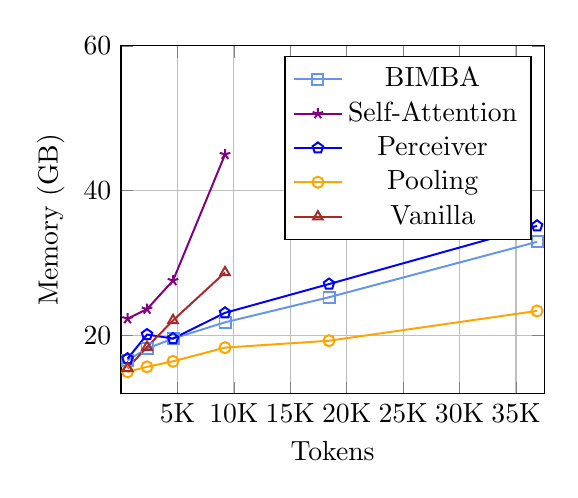
\begin{tikzpicture}
    \begin{axis}[
        height=6cm,
        xlabel={Tokens},
        ylabel={Memory (GB)},
        xmin=0, xmax=37500,
        ymin=12, ymax=60,
        xtick={5000, 10000, 15000, 20000,25000,30000, 35000},
        xticklabels={5K, 10K, 15K, 20K, 25K,30K, 35K},
        legend pos=north east,
        grid=both,
        scaled ticks = false,
        scaled x ticks = false,
    ]
    % BIMBA Data
    \addplot[line width=.25mm, color=CornflowerBlue, mark=square, mark size=2pt]
    coordinates {
    (576, 16.62) (2304, 18.22) (4608, 19.61) (9216, 21.85) (18432, 25.31) (36864, 32.95)
    };
    \addlegendentry{BIMBA}
    
    % Self-Attention Data
    \addplot[line width=.25mm, color=Purple, mark=star, mark size=2pt]
        coordinates {
        (576, 22.35) (2304, 23.67) (4608, 27.61) (9216, 45.01)
    };
    \addlegendentry{Self-Attention}

    % Perceiver Data
    \addplot[line width=.25mm,color=Blue, mark=pentagon, mark size=2pt]
    coordinates {
    (576, 16.83) (2304, 20.16) (4608, 19.61) (9216, 23.16) (18432, 27.13) (36864, 35.16)
    };
    \addlegendentry{Perceiver}
    
    % Pooling Data
    \addplot[line width=.25mm, color=Orange, mark=o, mark size=2pt]
    coordinates {
    (576, 15.02) (2304, 15.71) (4608, 16.47) (9216, 18.36) (18432, 19.31) (36864, 23.42)
    };
    \addlegendentry{Pooling}

    %Vanilla
    \addplot[line width=.25mm, color=Brown, mark=triangle, mark size=2pt]
    coordinates {
    (576, 15.51) (2304, 18.44) (4608, 22.12) (9216, 28.73) 
    };
    \addlegendentry{Vanilla}
    \end{axis}
    \end{tikzpicture}
    \caption{Memory Usage of Models based on LLaVA.}
    \vspace{1mm}
\end{subfigure}
\hfill
\begin{subfigure}[b]{0.45\textwidth}
    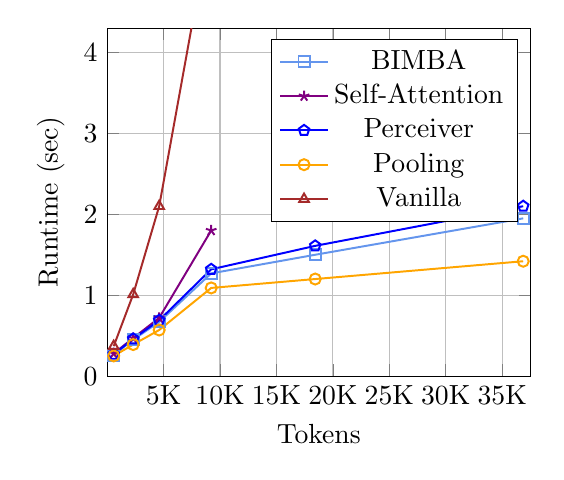
\begin{tikzpicture}
    \begin{axis}[
        % width=12cm, height=8cm,
        height=6cm,
        xlabel={Tokens},
        ylabel={Runtime (sec)},
        %title={(b) Runtime of models based on LLaVA},
        xmin=0, xmax=37500,
        ymin=0, ymax=4.3,
        %xtick={576, 2304, 4608, 9216, 18432, 36864},
        % xticklabels={576, 2304, 4608, 9216, 18432, 36864},
        xtick={5000, 10000, 15000, 20000,25000,30000, 35000},
        xticklabels={5K, 10K, 15K, 20K, 25K,30K, 35K},
        %ytick={43, 46, 49, 52, 55, 58, 61},
        legend pos=north east,
        grid=both,
        scaled ticks = false,
        scaled x ticks = false,
        % xmode=log,
        % log basis x=1
    ]
    % BIMBA Data
    \addplot[line width=.25mm, color=CornflowerBlue, mark=square, mark size=2pt]
    coordinates {
    (576, 0.26) (2304, 0.45) (4608, 0.67) (9216, 1.27) (18432, 1.50) (36864, 1.95)
    };
    \addlegendentry{BIMBA}
    
    % Self-Attention Data
    \addplot[line width=.25mm, color=Purple, mark=star, mark size=2pt]
        coordinates {
        (576, 0.28) (2304, 0.47) (4608, 0.72) (9216, 1.80)
    };
    \addlegendentry{Self-Attention}

    \addplot[line width=.25mm, color=Blue, mark=pentagon, mark size=2pt]
    coordinates {
    (576, 0.27) (2304, 0.46) (4608, 0.69) (9216, 1.32) (18432, 1.61) (36864, 2.1)
    };
    \addlegendentry{Perceiver}

    % Pooling Data
    \addplot[line width=.25mm, color=Orange, mark=o, mark size=2pt]
    coordinates {
    (576, 0.25) (2304, 0.39) (4608, 0.57) (9216, 1.09) (18432, 1.20) (36864, 1.42)
    };
    \addlegendentry{Pooling}

    %Vanilla
    \addplot[line width=.25mm, color=Brown, mark=triangle, mark size=2pt]
    coordinates {
    (576, 0.37) (2304, 1.01) (4608, 2.10) (9216, 5.65) 
    };
    \addlegendentry{Vanilla}
    
    \end{axis}
    \end{tikzpicture}
    \caption{Runtime of models based on LLaVA.}
    \vspace{1mm}
\end{subfigure}
\vspace{-4mm}
\caption{\small{Computation cost of \model { a}nd baseline models in terms of memory usage (left) and runtime (right). All models are based on LLaVA. Models based on self-attention or that do not perform compression (Vanilla) run quickly out of memory as the number of input tokens is increased. The runtime of \model { g}rows gracefully as a function of the input sequence length, unlike for the case of Vanilla.}}
\vspace{-5mm}
\label{fig:computation llava}
\end{figure*}